\subsection*{Partie I.}
\begin{enumerate}
  \item 
\begin{enumerate}
  \item Désignons par $\argsh$ la fonction proposée par l'énoncé avant d'avoir prouvé qu'elle est la bijection réciproque. Elle est définie dans $\R$ et strictement croissante comme somme et composée de fonctions croissantes. Elle est donc injective. De plus, pour tout réel $t$,
\begin{multline*}
\argsh(\sh(t)) = \ln\left( \sh(t) + \ch(t)\right) \; \left(\text{car } \ch(t)^2 - \sh(t)^2 = 1 \text{ et } \ch > 0\right) \\
=\ln(e^t) = t.
\end{multline*}
Cela signifie que $\argsh \circ \sh = \Id_\R$ ce qui montre que $\argsh$ est surjective donc bijective de bijection réciproque $\sh$. D'après la formule donnant la dérivée d'une bijection réciproque dérivable,
\begin{displaymath}
\forall x\in\R,\;  {\argsh}'(x) = \frac{1}{\ch(\argsh(x))} = \frac{1}{\sqrt{1+x^2}}.
\end{displaymath}

  \item Notons de même $\argch$ la fonction proposée. Elle est bien définie dans $[1,+\infty[$ (racine carrée) et strictement croissante (donc injective).\newline
De plus, pour tout réel $t\geq 0$,
\begin{displaymath}
\argsh(\ch(t)) = \ln\left( \sh(t) + \sh(t)\right) = \ln(e^t) = t.
\end{displaymath}
car $\ch(t)^2 - \sh(t)^2 = 1$ et $\sh(t) \geq 0$.\newline
Cela signifie que $\argch \circ \ch = \Id_{[0,+\infty[}$ donc $\argch$ est surjective donc bijective de bijection réciproque $\ch$ (restreinte à $[0,+\infty[$).\newline
D'après le résultat de cours sur la dérivée d'une bijection réciproque dérivable:
\begin{displaymath}
\forall x\geq 1,\;  {\argch}'(x) = \frac{1}{\sh(\argsh(x))} = \frac{1}{\sqrt{x^2 - 1}}.
\end{displaymath}
\end{enumerate}

  \item Comme sa partie réelle est strictement positive, le complexe $1+iu$ admet un argument $\alpha\in\left] -\frac{\pi}{2}, \frac{\pi}{2}\right[$ qui vérifie donc 
\begin{displaymath}
\left. 
\begin{aligned}
\sqrt{1+u^2}\cos \alpha &= 1 \\ \sqrt{1+u^2}\sin \alpha &= u  
\end{aligned}
\right\rbrace \Rightarrow \tan \alpha = u \Rightarrow \alpha = \arctan(u) .
\end{displaymath}
On en déduit la forme algébrique
\begin{displaymath}
  e^{i\theta(u)} = \frac{1+iu}{\sqrt{1+u^2}}.
\end{displaymath}

  \item D'après la forme algébrique précédente, on peut séparer la partie réelle et la partie imaginaire dans le calcul de l'intégrale de la fonction à valeurs complexes puis exprimer des primitives avec $\argch$ et $\argsh$.
\begin{displaymath}
x(t) = \int_0^{t}\frac{1}{\sqrt{1+u^2}}\,du =  \argsh(t) \hspace{0.5cm}
y(t) = \int_0^{t}\frac{u}{\sqrt{1+u^2}}\,du = \sqrt{1+t^2}-1 .
\end{displaymath}

  \item Rappelons que $t$ est positif.\newline
Expression de $t$ en fonction de $x(t)$.
\begin{displaymath}
x(t) = \argsh(t) \Rightarrow t = \sh(x(t)).
\end{displaymath}
Expression de $y(t)$ en fonction de $x(t)$.
\begin{displaymath}
y(t) = \sqrt{1+t^2}-1 = \sqrt{1+\sh(x(t))^2} -1 = \ch(x(t)) - 1 .
\end{displaymath}
On en déduit que les points d'affixes $z(t)$ sont sur la courbe représentative de $\ch -1$ limitée en abscisse aux réels positifs. Il s'agit de la demi-chaînette translatée verticalement. 
\end{enumerate}
\begin{figure}[h]
  \centering
  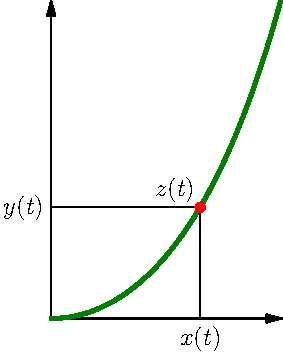
\includegraphics{./Celem18_1.pdf}
  % Celem18_1.pdf: 0x0 pixel, 300dpi, 0.00x0.00 cm, bb=
  \caption{demi-chaînette}
  \label{fig: Celem18_1}
\end{figure}


\subsection*{Partie II.}

\begin{enumerate}
\item Comme $\theta'$ est croissante, pour tout $t\in [0,+\infty[$, $\theta'(t)\geq \theta'(0) >0$. Intégrons $e^{i\theta(t)}$ par parties en remarquant que $\displaystyle{e^{i\theta(t)} = \frac{1}{i\theta'(t)}i\theta'(t)e^{i\theta(t)}}$. Posons:
\[ \left \{ \begin{array}{ll}
              f'(t) = i\theta'(t)e^{\theta(t)}\\
              g(t) = \frac{1}{i\theta'(t)}
            \end{array}
    \right.  \qquad \left \{ \begin{array}{ll}
                                f(t) = e^{i\theta(t)}\\
                                g'(t) = -\frac{\theta''(t)}{\theta'(t)}
                              \end{array}
                     \right. .
\]
On a alors:
\[
 z(t)  = -\int_{0}^{t} f(u)g'(u)\ du  + [f(u)g(u)]_{0}^{t}  
  = \int_{0}^{t}\frac{\theta''(u)}{i\theta'(u)^{2}}e^{i\theta(u)}\ du + \frac{e^{i\theta(t)}}{i\theta'(t)}-\frac{e^{i\theta(0)}}{i\theta'(0)}.
\]
 
\item D'après l'inégalité triangulaire:
\[ 
\abs{\frac{e^{i\theta(t)}}{i\theta'(t)}-\frac{e^{i\theta(0)}}{i\theta'(0)}} \leq \abs{\frac{e^{i\theta(t)}}{i\theta'(t)}}+\abs{\frac{e^{i\theta(0)}}{i\theta'(0)}} \leq \frac{1}{\theta'(t)} + \frac{1}{\theta'(0)}.  
\]
$\theta'(0) = \lambda$ et $\theta'(t)\geq \theta'(0) = \lambda$ donc:
\[
\abs{\frac{e^{i\theta(t)}}{i\theta'(t)}-\frac{e^{i\theta(0)}}{i\theta'(0)}} \leq \frac{2}{\lambda}.  
\]

\item D'après l'énoncé:
\[  
\abs{\int_{0}^{t}\frac{\theta''(u)}{i\theta'(u)^{2}}e^{i\theta(u)}\ du} 
\leq \int_{0}^{t}\abs{\frac{\theta''(u)}{i\theta'(u)^{2}}e^{i\theta(u)}}\ du. 
\]
Pour tout $u\in [0,t]$, $\theta(u)\in \R$ donc $\abs{e^{i\theta(u)}} = 1$. Comme $\theta'$ est croissante, $\theta''(u)\geq 0$. enfin, on a déjà vu que $\theta'(u)>0$, donc:
\[  
\abs{\int_{0}^{t}\frac{\theta''(u)}{i\theta'(u)^{2}}e^{i\theta(u)}\ du} \leq \int_{0}^{t}\frac{\theta''(u)}{\theta'(u)^{2}}\ du.  
\]

\item L'inégalité triangulaire et la question 1 donnent: 
\[ 
\abs{z(t)} \leq \abs{\int_{0}^{t}\frac{\theta''(u)}{\theta'(u)^{2}}e^{i\theta(u)}\ du} + \abs{\frac{e^{i\theta(t)}}{i\theta'(t)}-\frac{e^{i\theta(0)}}{i\theta'(0)}}.
\]
D'après la question 2 et la question 3, on a donc:
\[  
\abs{z(t)} \leq\int_{0}^{t}\frac{\theta''(u)}{\theta'(u)^{2}}\ du + \frac{2}{\lambda}.  
\]
L'intégrale se calcule:
\[ 
\int_{0}^{t}\frac{\theta''(u)}{\theta'(u)^{2}}\ du = \left [  -\frac{1}{\theta'(u)}   \right ]_{0}^{t} = \frac{1}{\theta'(0)}-\frac{1}{\theta'(t)}.  
\]
D'après l'inégalité triangulaire:
\[  
\abs{\int_{0}^{t}\frac{\theta''(u)}{\theta'(u)^{2}}\ du} \leq \frac{1}{\theta'(0)} + \frac{1}{\theta'(t)} \leq \frac{2}{\lambda}  
\]
puisque $\theta'(t)\geq \theta'(0) = \lambda$. On en déduit le résultat voulu:
\[  
\abs{z(t)}\leq \frac{4}{\lambda}.  
\]
\end{enumerate}
